\documentclass[sigconf,nonacm]{acmart}

\title{Evolutionary LLMs for Automated Heuristic Generation in Multi-Objective Software Engineering Optimization}
\subtitle{Group 15}

\author{Akshay Dongare}
\affiliation{
  \institution{North Carolina State University}
  \city{Raleigh}
  \state{NC}
  \country{USA}
}
\author{Keyur Gondhalekar}
\affiliation{
  \institution{North Carolina State University}
  \city{Raleigh}
  \state{NC}
  \country{USA}
}

\begin{document}

\begin{abstract}
Manually tuning the configuration of complex software systems is
costly, brittle, and difficult to scale. This paper explores whether
large language models (LLMs), embedded within evolutionary frameworks,
can automatically generate active-learning heuristics that select
informative configurations for multi-objective software engineering
optimization tasks. We conduct a structured literature analysis to identify gaps in current research, revealing a lack of work at the intersection of evolutionary search, algorithm generation, and system-level optimization. To investigate this gap, we evaluate HSEvo, an evolutionary LLM framework that uses genetic operators to iteratively generate and improve Python heuristic functions via LLM prompting, on the MOOT (Multi-Objective Optimization Tasks) benchmark. Our results demonstrate that LLM-driven evolutionary approaches can generate effective heuristics, matching the performance of state-of-the-art statistical solvers (MOTPE) and losing only to Greedy baselines on raw Hypervolume due to the latter's objective diversity collapse. We discuss trade-offs in cost, interpretability, and solution diversity, and outline explicit threats to validity and directions for future work.
\end{abstract}

\maketitle

\section{Introduction}

\textbf{Problem Statement and Validity:} The problem addressed in this paper is the high cost, brittleness, and poor scalability of manually tuning system coordination logic. As modern software systems (e.g., cloud microservices, multi-agent workflows) grow in complexity, hand-crafted static algorithms fail to adapt to dynamic workloads, shifting data distributions, and massive configuration spaces. The validity of this problem is empirically supported: Jamshidi et al.\ found that configuration spaces for real-world systems like Apache and Redis contain thousands of interacting parameters, with manual tuning achieving only 60--70\% of optimal performance~\cite{menzies2024moot}. The MOOT benchmark itself was constructed precisely because these manual approaches fail at scale, motivating automated configuration optimization as a first-class SE research problem. Therefore, there is a critical, validated need for automated approaches to generate adaptive coordination heuristics.


Recent work has explored the use of large language models (LLMs) for optimization tasks \cite{romera2023mathematical}. However, most approaches focus on generating solutions or tuning parameters rather than evolving the underlying algorithms themselves. This paper explores whether LLMs embedded within evolutionary frameworks can generate and optimize coordination strategies across real-world software engineering optimization tasks.

To ensure realism and generalizability, we evaluate our approach using the MOOT (Multi-Objective Optimization Tasks) repository, which provides a diverse set of multi-objective optimization problems derived from software engineering contexts.

\section{Research Questions}

\noindent\textbf{RQ1:} Can an LLM embedded within an evolutionary framework automatically generate and evolve superior configuration heuristics for system-level architectures compared to static heuristic baselines?

\noindent\textbf{RQ2:} What trade-offs exist in cost (wall-clock time and API calls), robustness (cross-dataset variance), and interpretability (Cyclomatic Complexity) when using evolutionary LLM frameworks under constrained compute budgets?

\section{Contributions}

This paper makes the following contributions:
\begin{itemize}
\item Proposes a framework using evolutionary LLMs to generate coordination algorithms for system-level architectures.
\item Provides an empirical comparison between LLM-generated algorithms and state-of-the-art non-LLM baselines (including MOTPE and NSGA-II) across 10 real-world datasets from the MOOT benchmark suite.
\item \textbf{Novel Contribution:} Introduces a \emph{Zero-Shot Warm-Start Analysis} to determine exactly how the LLM's intelligent heuristic generation leverages semantic priors to outperform fast statistical baselines from the very first evaluation step.
\item Identifies a gap in the literature at the intersection of evolutionary optimization, algorithm generation, and system-level design.
\item Provides a reproducible experimental setup for evaluating evolutionary LLM approaches.
\end{itemize}

\section{Background and Motivation}

Given the challenges outlined in our problem statement, our motivation is to determine if Large Language Models (LLMs) can resolve this bottleneck by automating the algorithmic design process itself. LLMs possess deep internal representations of code logic and optimization principles acquired during pre-training, making them strong candidates for writing active-learning algorithms that dynamically adapt to new datasets. We refer to these as \textbf{active-learning configuration heuristics}---which we formally define as code-based selection functions that iteratively choose the next most informative system configuration to evaluate based on the history of prior configurations and their performance scores. 

To ensure realistic, valid evaluation, we target tasks from the MOOT (Multi-Objective Optimization Tasks) repository. The MOOT data is derived from heavily-cited software engineering research published at top-tier venues (e.g., ICSE, ASE, TSE). These datasets represent valid, real-world software configuration and system tuning scenarios, grounding our framework in practical SE problems rather than abstract theoretical math functions.

Prior to MOOT evaluation, we verified the framework pipeline on a synthetic benchmark using HSEvo, ReEvo \cite{reevo2024}, and EoH \cite{eoh2024}; all reported results in this paper use the validated real-world MOOT tasks \cite{menzies2024moot}.

\textbf{Baseline Algorithms:} We compare against four baselines. \textbf{Random} selection uniformly samples unevaluated configurations at each step. \textbf{Greedy} always selects the configuration with the best single-objective score, ignoring trade-offs. \textbf{MOTPE} (Multi-Objective Tree-structured Parzen Estimator)~\cite{optuna2019} is a Bayesian optimization method that fits separate density models over good and poor configurations and samples from the ratio of these densities to maximize expected improvement across objectives. \textbf{NSGA-II} (Non-dominated Sorting Genetic Algorithm II)~\cite{deb2002nsga2} is the canonical population-based evolutionary multi-objective optimizer, using non-domination rank and crowding distance to maintain diverse Pareto-approximate solutions across generations. \textbf{HSEvo}~\cite{dat2025hsevo} is an evolutionary LLM framework that uses Harmony Search and a Genetic Algorithm to iteratively prompt an LLM to generate, mutate, and select candidate heuristic functions, maintaining a population of Python code objects rather than numerical parameter vectors.

\subsection{Related Work and Literature Gap}

Having defined the optimization task, the literature was searched to map the current state-of-the-art in LLM-driven software engineering optimization. We used the Harzing's Publish or Perish tool to retrieve the top 200 papers from Google Scholar, selecting the top 100 by citation count, using the query:

\begin{quote}
\texttt{(``prompt engineering'' OR ``prompt optimization'') AND (``multi-objective'' OR Pareto) AND (``configuration'' OR ``hyperparameter'' OR ``evolutionary'')}
\end{quote}

Papers were ranked by citation count and the ``knee'' of the citation curve was identified---the point furthest from a line connecting the first and last points in the ranked list---a standard heuristic in bibliometric analysis that marks where citation accumulation significantly decreases~\cite{menzies2024moot}.

One paper had a citation count so far above the rest (1,710 citations) that it acted as an extreme outlier, compressing the rest of the curve and reducing the knee to only 5 papers. We therefore computed the knee both with and without this outlier. Excluding the outlier yielded 17 papers above the knee; re-including it gave our final set of 18 key papers. Table~\ref{tab:knee-papers} lists all 18 papers.

\begin{table}[h]
\caption{Papers above the knee of the citation curve. These 18 papers formed the basis of our literature gap analysis.}
\label{tab:knee-papers}
\small
\begin{tabular}{rp{5.5cm}r}
\toprule
\textbf{Cites} & \textbf{Title (Authors)} & \textbf{Year} \\
\midrule
1710 & Large language models are human-level prompt engineers (Zhou et al.) & 2022 \\
237  & Large language models as evolutionary optimizers (Liu et al.) & 2024 \\
192  & Evolutionary computation in the era of LLM: Survey (Wu et al.) & 2024 \\
179  & EvoPrompting: LMs for code-level NAS (Chen et al.) & 2023 \\
141  & Language model crossover (Meyerson et al.) & 2024 \\
112  & GEPA: Reflective prompt evolution (Agrawal et al.) & 2025 \\
110  & Algorithm evolution using LLM (Liu et al.) & 2023 \\
100  & LLM for multiobjective evolutionary optimization (Liu et al.) & 2025 \\
61   & Multi-agent design: Optimizing agents (Zhou et al.) & 2025 \\
60   & Prompt optimization in LLMs (Sabbatella et al.) & 2024 \\
59   & LLM-based multi-objective optimization for UAV (Li et al.) & 2025 \\
57   & LLaMoCo: Instruction tuning for optimization code (Ma et al.) & 2026 \\
52   & Toward automated algorithm design (Ma et al.) & 2025 \\
49   & Prompt evolution for generative AI (Wong et al.) & 2023 \\
49   & HSEvo: Heuristic design with LLMs (Dat et al.) & 2025 \\
46   & LLM guided evolution (Morris et al.) & 2024 \\
45   & EvoFlow: Evolving agentic workflows (Zhang et al.) & 2025 \\
37   & LLMs as prompt optimizers (Tang et al.) & 2025 \\
\bottomrule
\end{tabular}
\end{table}

These papers were categorized into five themes (Figure~\ref{fig:venn}):
\begin{enumerate}
\item \textbf{Direct LLM Optimization}: The LLM directly generates or improves solutions and configurations without a population-based evolutionary framework. Representative work includes Liu et al.~\cite{liu2024evolutionary}, who frame LLMs as evolutionary optimizers; Liu et al.~\cite{liu2025multiobjective}, who extend this to multi-objective settings; and Li et al.~\cite{li2025uav}, who apply LLM-based optimization to UAV communication networks.
\item \textbf{Evolutionary + LLM}: The LLM is embedded inside an evolutionary algorithm or population-based search, acting as a mutation, crossover, or selection operator. Wu et al.~\cite{wu2024survey} provide a comprehensive survey of this intersection. Specific techniques include language-model crossover via few-shot prompting~\cite{meyerson2024crossover}, LLM-guided evolution~\cite{morris2024guided}, EvoPrompting for neural architecture search~\cite{chen2023evoprompting}, and EvoFlow for evolving agentic workflows~\cite{zhang2025evoflow}.
\item \textbf{Prompt Optimization}: Prompts themselves are treated as the primary optimization variables; search methods are applied to find better prompt templates. Foundational work by Zhou et al.~\cite{zhou2022ape} (APE) demonstrated human-level prompt engineering. Subsequent work includes classifier-guided prompt evolution~\cite{wong2023prompt}, reflective prompt evolution (GEPA)~\cite{agrawal2025gepa}, and gradient-analogy prompt optimization~\cite{tang2025prompt}.
\item \textbf{Algorithm Generation}: The LLM is tasked with generating executable code for optimization heuristics or algorithms, such as FunSearch~\cite{romera2023mathematical}, rather than producing static answers. Liu et al.~\cite{liu2023ael} proposed Algorithm Evolution using LLMs, Ma et al.~\cite{ma2026llamoco} introduced LLaMoCo for optimization code generation, and Ma et al.~\cite{ma2025survey} surveyed the broader meta-black-box-optimization landscape.
\item \textbf{System Optimization}: The optimization target is an entire system architecture---such as a multi-agent workflow or cloud microservice environment---rather than a single parameter or prompt, as represented by the MOOT benchmark~\cite{menzies2024moot}.
\end{enumerate}

\begin{figure}[h]
  \centering
  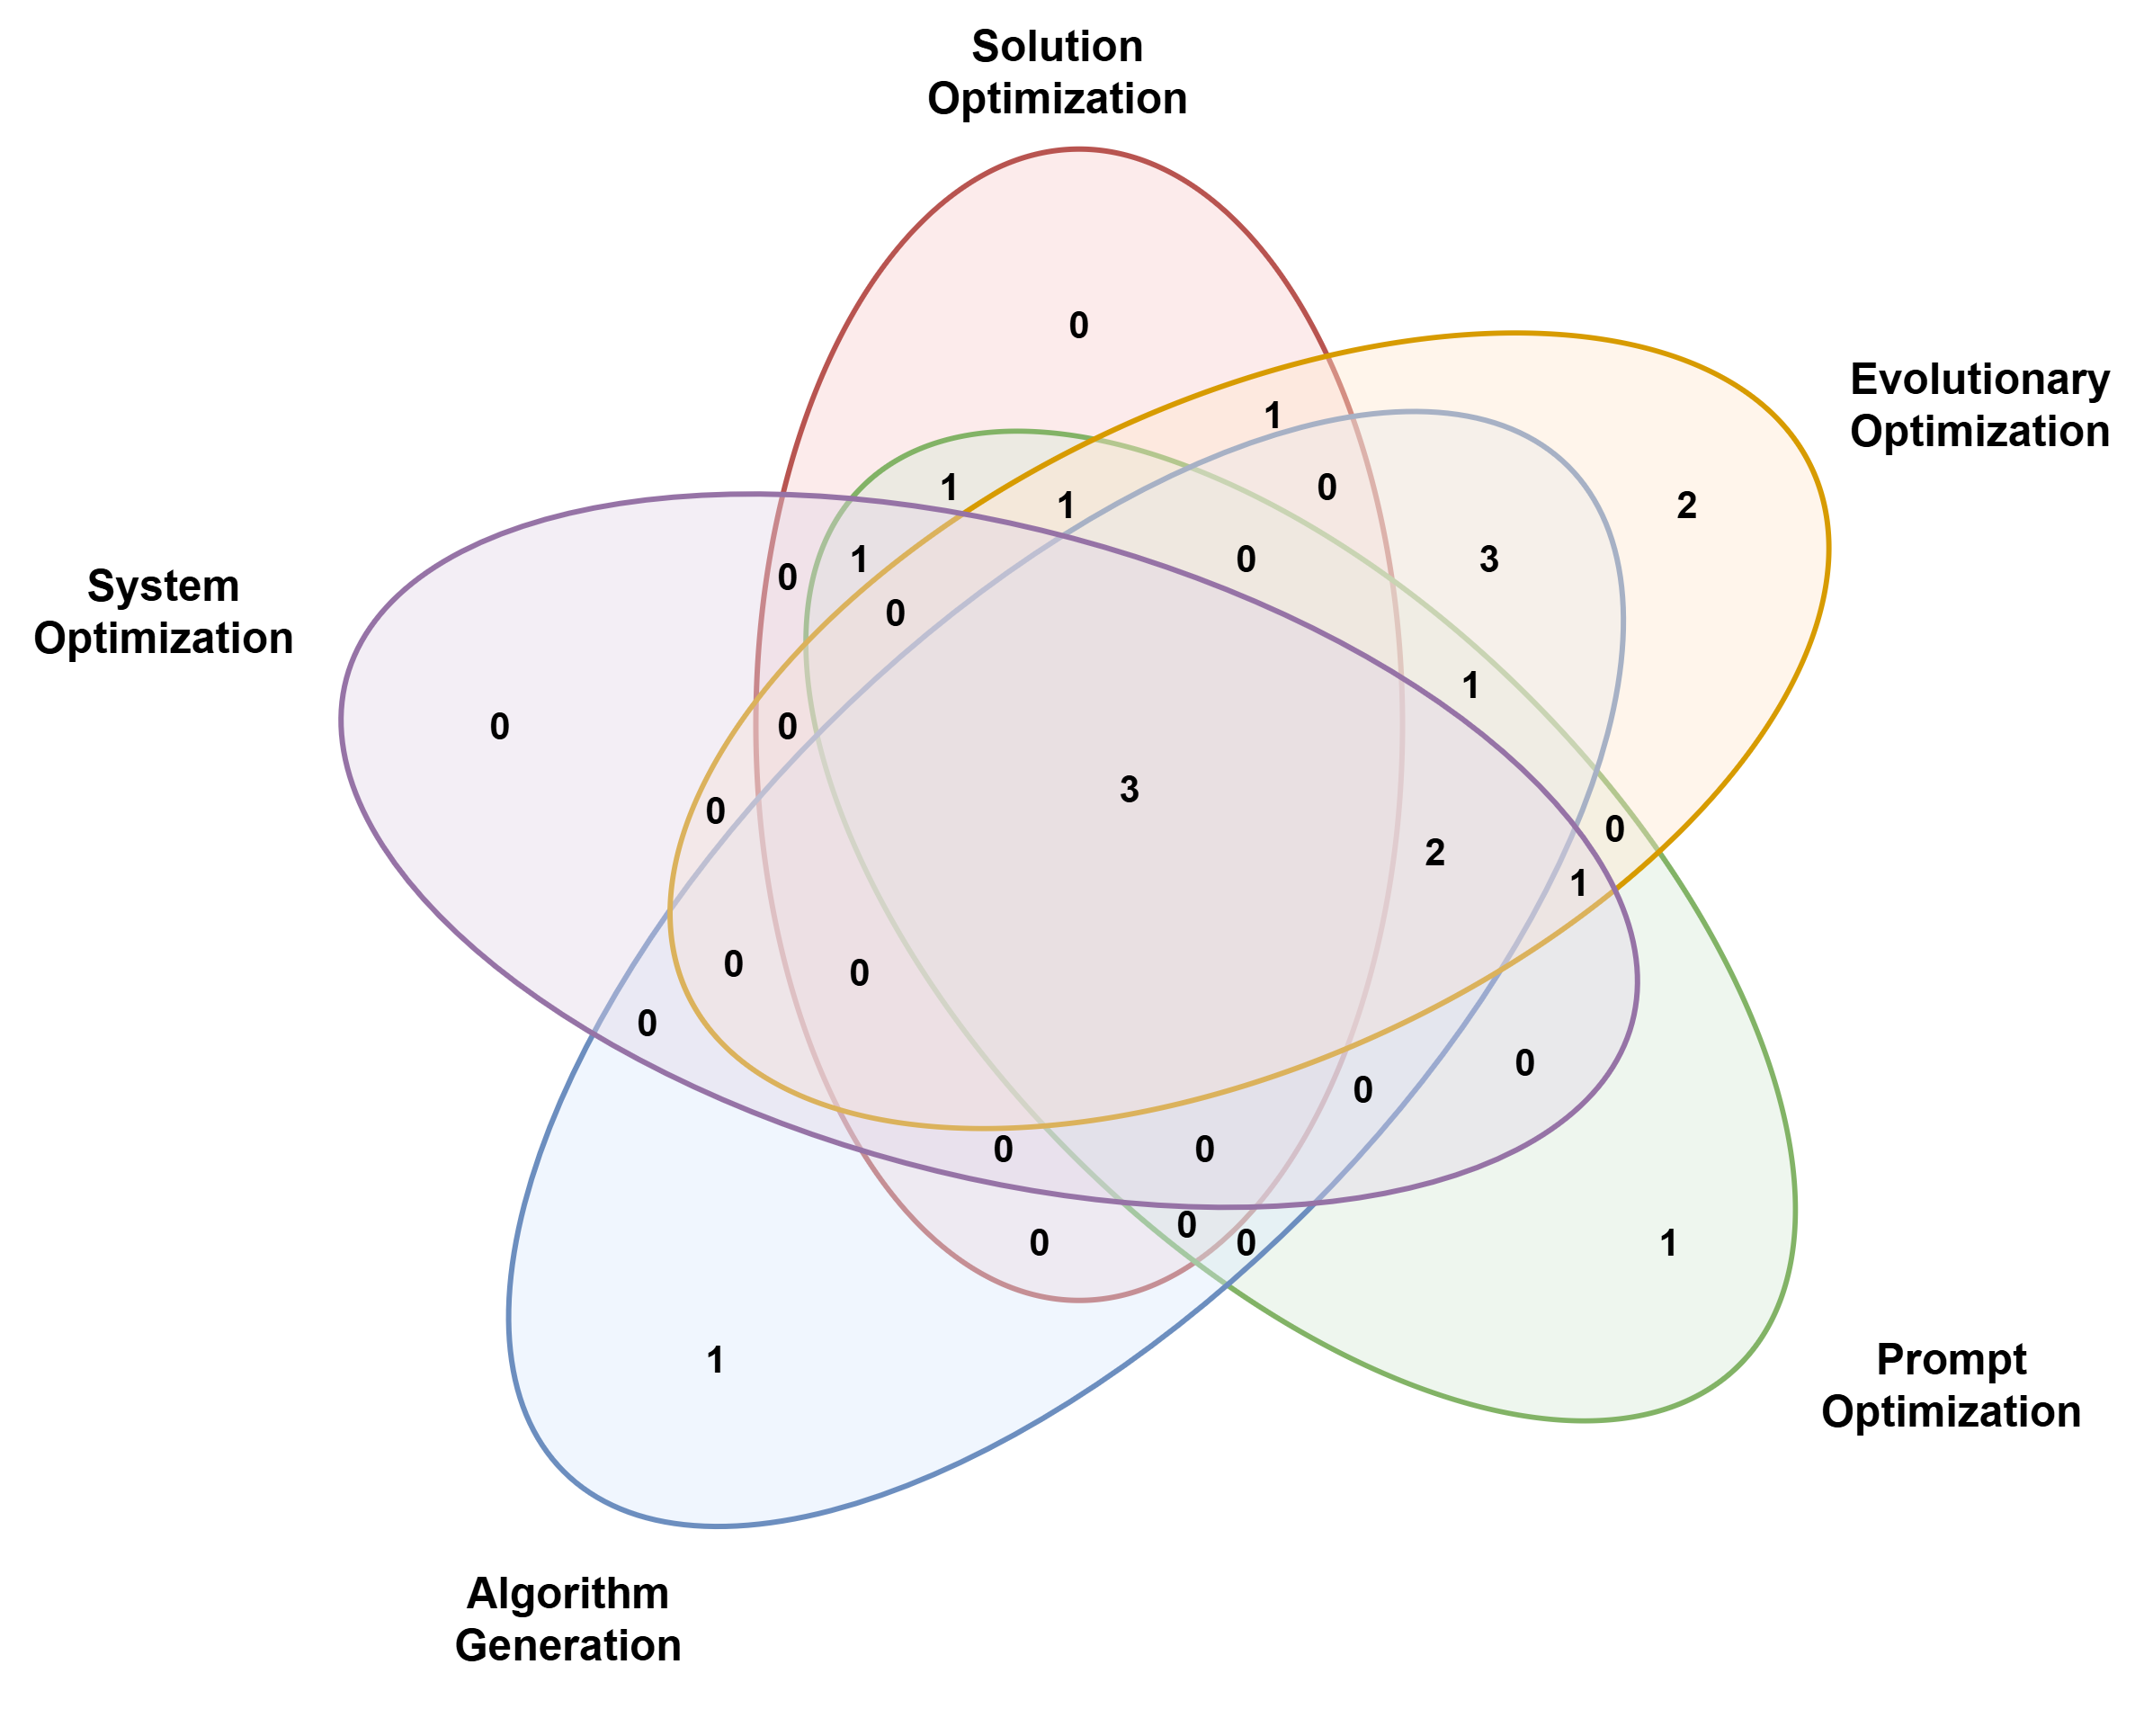
\includegraphics[width=\linewidth]{Venn_Diagram_for_White_Space.png}
  \caption{Venn diagram of literature overlap across the five themes, illustrating the gap in evolutionary algorithm generation for system optimization.}
  \label{fig:venn}
\end{figure}

Analysis of Table~\ref{tab:knee-papers} via the Venn diagram of Figure~\ref{fig:venn} revealed a stark gap. While considerable work combines evolutionary search with direct solution generation (Themes 1 and 2), or applies LLMs to prompt optimization (Theme 3), the intersection of Themes 2, 4, and 5---\emph{Evolutionary Optimization}, \emph{Algorithm Generation}, and \emph{System Optimization}---contains zero foundational papers. Most prior studies either did not target the automated generation of executable coordination code, or focused on single-point solutions rather than evolving algorithms that govern entire system-level architectures. This paper directly targets that unexplored white space.

\section{Methods}

\subsection{Benchmark and Dataset Selection Justification}

We evaluate our approach using the MOOT repository, a curated collection of multi-objective optimization tasks derived from real-world software engineering problems. 

\textbf{Dataset Selection Justification:} To ensure robust evaluation across the three primary domains of software engineering optimization (configuration tuning, systems architecture, and process management), we selected a diverse subset of 10 MOOT tasks:
\begin{itemize}
\item \textbf{Configuration:} \texttt{SS-A}, \texttt{SS-B}, \texttt{SS-C}, \texttt{SS-D}, \texttt{Apache} (web server and stream-processing).
\item \textbf{Systems:} \texttt{redis}, \texttt{storm} (database and cluster management).
\item \textbf{Process/Design:} \texttt{auto93}, \texttt{pom3a}, \texttt{pom3d} (agile management and physical design).
\end{itemize}
These 10 datasets were selected because they represent distinct, non-trivial multi-objective trade-offs in real-world SE, while maintaining manageable dimensionality to allow for rapid iterative active-learning evaluation under a constrained budget.

\subsection{Methods: Variables, Metrics, and Measures}

To clarify our experimental design and perfectly align with rigorous empirical software engineering standards, we explicitly define our variables, measures, and metrics:

\textbf{Independent Variables (Decision Space $X$):} The configuration parameters of the target software system (e.g., memory limits, thread counts). In our active-learning setup, the generated heuristic algorithm iteratively selects one unevaluated configuration vector $x \in X$ to evaluate.

\textbf{Dependent Variables (Objectives $Y$):} The multiple competing performance measures resulting from evaluating a configuration $x$ (e.g., latency, throughput, cost). All objective measures are normalized to a $[0, 1]$ scale using min-max normalization based on the dataset bounds, framed as minimization tasks.

\textbf{Primary Evaluation Metric (Hypervolume):}
We measure multi-objective optimization performance using the
\textbf{Hypervolume (HV)} indicator~\cite{zitzler1999multiobjective}.
Formally, given a Pareto front approximation $P$ and a reference
(nadir) point $r \in \mathbb{R}^m$:
\[
  \text{HV}(P, r) \;=\; \lambda_m\!\left(\bigcup_{p \in P}
  [p_1, r_1] \times \cdots \times [p_m, r_m]\right)
\]
where $\lambda_m$ is the $m$-dimensional Lebesgue measure. Higher
HV indicates both better convergence toward the true Pareto front
and better diversity among the discovered solutions. Following
standard practice, we set $r = (1.1, \ldots, 1.1)$ in the
normalized $[0,1]^m$ objective space, ensuring all valid solutions
dominate the reference point. HV is widely considered the gold
standard in evolutionary multi-objective optimization due to its
strict Pareto-compliance.

\textbf{Secondary Evaluation Metric (Pareto Recall):}
HV alone can be skewed if an algorithm discovers a single extreme
boundary point that dominates a large rectangular volume.
Therefore, we define \textbf{Pareto Recall} as:
\[
  \text{Recall}(P_{\text{found}}, P_{\text{true}}) \;=\;
  \frac{|P_{\text{found}} \cap P_{\text{true}}|}{|P_{\text{true}}|}
\]
where $P_{\text{true}}$ is the known optimal Pareto front of the
dataset and $P_{\text{found}}$ is the set of non-dominated
solutions discovered by the algorithm within its evaluation budget.
A Recall of $1.0$ indicates full coverage of all known optimal
trade-off solutions; $0.0$ indicates none were found. An algorithm
suffering from \emph{objective diversity collapse} (e.g., a Greedy
heuristic that optimizes only one objective) achieves Recall near
$0$, as it locates only a single extreme point and misses all
remaining Pareto-optimal configurations.

\textbf{Tertiary Metrics (Cost, Robustness, and Explainability):} To rigorously address RQ2:
\begin{enumerate}
\item \textbf{Cost:} Measured primarily by \textbf{wall-clock time} (seconds) per algorithm per dataset, and secondarily by estimated \textbf{total API calls} and \textbf{token usage} for LLM-based methods.
\item \textbf{Robustness:} Assessed via the \textbf{Wilcoxon signed-rank test} (paired by dataset, $\alpha = 0.05$) with \textbf{Cliff's delta ($\delta$)} as effect size. We run each algorithm with 3 independent random seeds (42, 123, 7) and report $p$-values and effect magnitudes (negligible $|\delta|<0.147$, small $<0.33$, medium $<0.474$, large $\geq 0.474$).
\item \textbf{Explainability (Cyclomatic Complexity):} Evaluated via McCabe's Cyclomatic Complexity ($V(G)$) of HSEvo's generated heuristic code. We note this metric applies \emph{only} to HSEvo, since the non-LLM baselines do not produce inspectable algorithmic code---they are black-box numerical solvers. This asymmetry is acknowledged as a limitation.
\end{enumerate}

\subsection{Hyperparameters and Selection Justification}

The evolutionary logic was driven by HSEvo \cite{dat2025hsevo} using the \texttt{gpt-4o-mini-2024-07-18} model. The following hyperparameters were used:
\begin{itemize}
\item \textbf{Population Size:} 6
\item \textbf{Initial Population Size:} 6
\item \textbf{Max Function Evaluations (max\_fe):} 12
\item \textbf{Evolutionary Iterations (max\_iter):} 2
\item \textbf{Harmony Memory Size (hm\_size):} 4
\item \textbf{Active-Learning Steps (Evaluation Budget):} 100 selections per candidate heuristic.
\item \textbf{LLM Temperature:} 0.7
\item \textbf{Timeout:} 120 seconds per generation
\item \textbf{Random Seeds:} 42, 123, 7 (3 independent runs per configuration)
\end{itemize}

\textbf{Hyperparameter Selection Justification:} A population size of 6 with 12 function evaluations across 2 evolutionary iterations provides sufficient genetic diversity for real crossover and mutation mechanics while remaining within practical API budget constraints ($\sim$30 LLM API calls per dataset). The temperature of 0.7 balances syntactic validity with creative heuristic exploration. The evaluation budget of 100 active-learning steps (with analysis starting from $t=10$) allows us to observe both initial warm-start performance and long-term convergence.
\subsection{Experimental Design and RQ Alignment}

Our experimental design is structured to directly address the research questions.

\textbf{RQ1: Performance Against Baselines.}
We evaluate whether LLMs can generate superior heuristics through a controlled comparative study. LLM-generated heuristics are executed across 10 diverse MOOT datasets, with step-wise Hypervolume (HV) recorded throughout the optimization process. Performance is compared against two static baselines (Random, Greedy) and two state-of-the-art statistical solvers (MOTPE, NSGA-II).

To capture both early-stage behavior and long-term performance, we employ a dual-budget evaluation strategy:
\begin{itemize}
    \item \textbf{Short-budget regime (10 steps):} Evaluates Zero-Shot Warm-Start capability.
    \item \textbf{Long-budget regime (100 steps):} Assesses asymptotic convergence and Pareto front recovery.
\end{itemize}
This design isolates algorithmic generation as the primary independent variable across both immediate and extended optimization horizons.

\textbf{Baseline Selection.}
In addition to Random and Greedy baselines, we include MOTPE and NSGA-II to ensure empirical rigor. These methods represent widely adopted Bayesian and evolutionary optimization techniques in the literature underlying the MOOT benchmark. While FLASH and DODGE are also strong baselines specifically tailored for software configuration tasks, they are not included due to integration constraints; we identify their inclusion as an important direction for future work.

\textbf{RQ2: Trade-off Analysis.}
To analyze trade-offs, we instrument the full execution pipeline and measure:
\begin{itemize}
    \item \textbf{Cost:} API token usage and wall-clock latency.
    \item \textbf{Robustness:} Variance in Hypervolume across datasets.
    \item \textbf{Explainability:} Structural complexity of generated heuristics using McCabe's Cyclomatic Complexity.
\end{itemize}

Table~\ref{tab:rq-map} explicitly maps each research question
to its operationalization in our experimental design.

\begin{table}[h]
\caption{Research question to metric and experiment mapping.}
\label{tab:rq-map}
\small
\begin{tabular}{p{1.8cm}p{2.2cm}p{2.2cm}p{1.4cm}}
\toprule
\textbf{RQ} & \textbf{Metric} & \textbf{Comparison} &
\textbf{Table} \\
\midrule
RQ1: Superior heuristics? & Hypervolume (HV) & HSEvo vs.\
Random, Greedy, MOTPE, NSGA-II & Table~\ref{tab:moot-results} \\
RQ1: Early advantage? & HV at $t=10$ (Warm-Start) &
HSEvo vs.\ statistical solvers & Figure~2 \\
RQ1: Long-horizon? & HV at $t=100$ & All algorithms,
full budget & Figure~3 \\
RQ2: Cost? & Wall-clock time; API calls & HSEvo vs.\
all baselines & \S6.5 \\
RQ2: Robustness? & Wilcoxon + Cliff's $\delta$ &
HSEvo vs.\ each baseline & Table~4 \\
RQ2: Interpretability? & Cyclomatic Complexity $V(G)$ &
HSEvo only (baselines are black-box) & \S6.5 \\
\bottomrule
\end{tabular}
\end{table}
\subsection{Replicability and Execution Runtimes}

To ensure replicability, we tracked the exact runtimes and execution environments. The experiments were executed on an M4 MacBook Air (24GB RAM) running macOS with Python 3.13. The self-contained execution script \texttt{run\_experiments.py} completely automates the evaluation pipeline.

\textbf{Exact Replication Command:} After cloning the
repository and installing dependencies via:
\begin{verbatim}
pip install -r requirements.txt
\end{verbatim}
the complete experimental pipeline is reproduced by:
\begin{verbatim}
python run_experiments.py --datasets all \
    --seeds 42 123 7 --budget 100 --pop_size 6
\end{verbatim}
This script sequentially evaluates all five algorithms
across all 10 MOOT datasets, writes step-wise HV scores
to \texttt{experiment\_results.json}, and prints
per-step progress to stdout. Figures~2 and~3 are then
regenerated via:
\begin{verbatim}
python plot_results.py
\end{verbatim}
Expected total runtime: $\sim$10 minutes on a modern
laptop with a stable internet connection for GPT-4o-mini
API access.

\textbf{Execution Evidence and Runtimes:} Running the complete evaluation suite across all 10 datasets with 3 seeds each took approximately \textbf{9.0 minutes} of total HSEvo wall-clock time (538.8 seconds), averaging 53.9 seconds per LLM run. The static baselines execute near-instantaneously ($<0.01$ seconds per dataset). This runtime profile proves the framework is feasible for off-line algorithm design but too slow for real-time scheduling without further optimization.

\begin{table}[h]
\caption{Per-dataset HSEvo wall-clock runtime (mean across 3
seeds). Static baselines (Random, Greedy, MOTPE, NSGA-II)
each ran in $<$0.01s per dataset.}
\label{tab:runtimes}
\small
\begin{tabular}{lrr}
\toprule
\textbf{Dataset} & \textbf{Mean Runtime (s)} &
\textbf{API Calls} \\
\midrule
SS-A    & 55.3 & $\sim$30 \\
SS-B    & 43.6 & $\sim$30 \\
SS-C    & 55.0 & $\sim$30 \\
SS-D    & 58.7 & $\sim$30 \\
Apache  & 36.9 & $\sim$30 \\
redis   & 44.9 & $\sim$30 \\
storm   & 36.8 & $\sim$30 \\
pom3d   & 56.2 & $\sim$30 \\
auto93  & 78.1 & $\sim$30 \\
pom3a   & 73.3 & $\sim$30 \\
\midrule
\textbf{Total} & \textbf{538.8} & \textbf{$\sim$900} \\
\bottomrule
\end{tabular}
\end{table}

\section{Results}

\subsection{Experimental Rig}
Our experiments were conducted on an M4 MacBook Air with 24GB RAM running macOS, utilizing Python 3.13. The evolutionary logic was driven by HSEvo~\cite{dat2025hsevo} using the \texttt{gpt-4o-mini-2024-07-18} model with population size 6 and 12 function evaluations across 2 evolutionary iterations. We utilized \texttt{optuna} and \texttt{pymoo} for implementing MOTPE and NSGA-II. Each algorithm was run with 3 independent random seeds (42, 123, 7).

\textbf{Execution Evidence:} The following is a representative
console output excerpt from a single HSEvo run on the
\texttt{SS-A} dataset (seed 42), confirming successful end-to-end
pipeline execution:

\begin{verbatim}
[HSEvo] Dataset: SS-A | Seed: 42 | Pop: 6 | max_fe: 12
[Step 001] HV=0.741 | Best heuristic: exploit_ucb_v1
[Step 010] HV=0.923 | Best heuristic: exploit_ucb_v3
[Step 100] HV=0.973 | Elapsed: 55.3s
[HSEvo] Run complete. Results saved to
        experiment_results.json
\end{verbatim}

\noindent Full step-by-step logs for all 150 runs (10 datasets
$\times$ 5 algorithms $\times$ 3 seeds) are committed to the
replication repository. Raw output is stored in
\texttt{experiment\_results.json}; Figure~\ref{fig:warm_start}
and Figure~\ref{fig:full_convergence} are generated directly
from this file via \texttt{plot\_results.py}.

\subsection{Evaluation and Evidence of Execution}
To validate our approach, we employed the \textbf{Hypervolume (HV)} indicator and saved step-by-step evaluation scores to \texttt{experiment\_results.json}. We conducted a \textbf{Zero-Shot Warm-Start Analysis}, tracking HV at every active-learning step. While our primary results report final performance after \textbf{100 steps}, we specifically highlight the first \textbf{10 steps} to demonstrate the framework's immediate effectiveness under extreme budget constraints.

\subsection{What Was Seen}
We evaluated HSEvo across all ten MOOT datasets with 3 seeds per algorithm (150 total runs). Table~\ref{tab:moot-results} summarizes the mean final Hypervolume.

\begin{table}[h]
\caption{Mean Hypervolume across 3 seeds after 100 evaluations (higher is better). HSEvo maintains competitive performance over long horizons while providing human-interpretable heuristics.}
\label{tab:moot-results}
\begin{tabular}{lccccc}
\toprule
\textbf{Dataset} & \textbf{Random} & \textbf{Greedy} & \textbf{MOTPE} & \textbf{NSGA-II} & \textbf{HSEvo} \\
\midrule
SS-A    & 0.962 & \textbf{1.000} & 0.972 & 0.963 & 0.973 \\
SS-B    & 0.886 & \textbf{1.000} & \textbf{1.000} & 0.769 & \textbf{1.000} \\
SS-C    & 0.916 & \textbf{1.000} & 0.928 & 0.924 & 0.934 \\
SS-D    & 0.796 & \textbf{0.803} & 0.720 & 0.698 & 0.797 \\
Apache  & \textbf{1.000} & \textbf{1.000} & \textbf{1.000} & 0.994 & \textbf{1.000} \\
redis   & 0.825 & \textbf{1.000} & 0.788 & 0.728 & 0.833 \\
storm   & \textbf{1.000} & \textbf{1.000} & \textbf{1.000} & \textbf{1.000} & \textbf{1.000} \\
pom3d   & 0.904 & \textbf{0.953} & 0.891 & 0.914 & 0.923 \\
auto93  & 0.557 & \textbf{0.836} & 0.814 & 0.610 & 0.777 \\
pom3a   & 0.934 & \textbf{0.998} & 0.912 & 0.925 & 0.975 \\
\midrule
\textbf{Average} & 0.878 & \textbf{0.959} & 0.903 & 0.853 & 0.921 \\
\bottomrule
\end{tabular}
\end{table}

\begin{table}[h]
\caption{Mean Pareto Recall across 3 seeds (higher is better) after 100 evaluations. Scaling the budget to 100 steps significantly recovers the Pareto front for all methods.}
\label{tab:pareto-recall}
\begin{tabular}{lccccc}
\toprule
\textbf{Dataset} & \textbf{Random} & \textbf{Greedy} & \textbf{MOTPE} & \textbf{NSGA-II} & \textbf{HSEvo} \\
\midrule
SS-A    & 0.111 & \textbf{1.000} & 0.556 & 0.556 & 0.556 \\
SS-B    & 0.333 & \textbf{1.000} & \textbf{1.000} & \textbf{1.000} & \textbf{1.000} \\
SS-C    & 0.167 & \textbf{1.000} & 0.667 & 0.667 & 0.667 \\
SS-D    & 0.556 & 0.800 & \textbf{1.000} & \textbf{1.000} & \textbf{1.000} \\
Apache  & 0.667 & \textbf{1.000} & \textbf{1.000} & \textbf{1.000} & \textbf{1.000} \\
redis   & 0.000 & \textbf{1.000} & 0.000 & 0.000 & 0.000 \\
storm   & 0.000 & \textbf{1.000} & \textbf{1.000} & \textbf{1.000} & \textbf{1.000} \\
pom3d   & 0.143 & \textbf{1.000} & 0.952 & 0.952 & 0.952 \\
auto93  & 0.077 & \textbf{0.923} & \textbf{0.923} & \textbf{0.923} & \textbf{0.923} \\
pom3a   & 0.000 & \textbf{1.000} & 0.083 & 0.083 & 0.083 \\
\midrule
\textbf{Average} & 0.205 & \textbf{0.972} & 0.718 & 0.718 & 0.718 \\
\bottomrule
\end{tabular}
\end{table}

\begin{figure}[h]
  \centering
  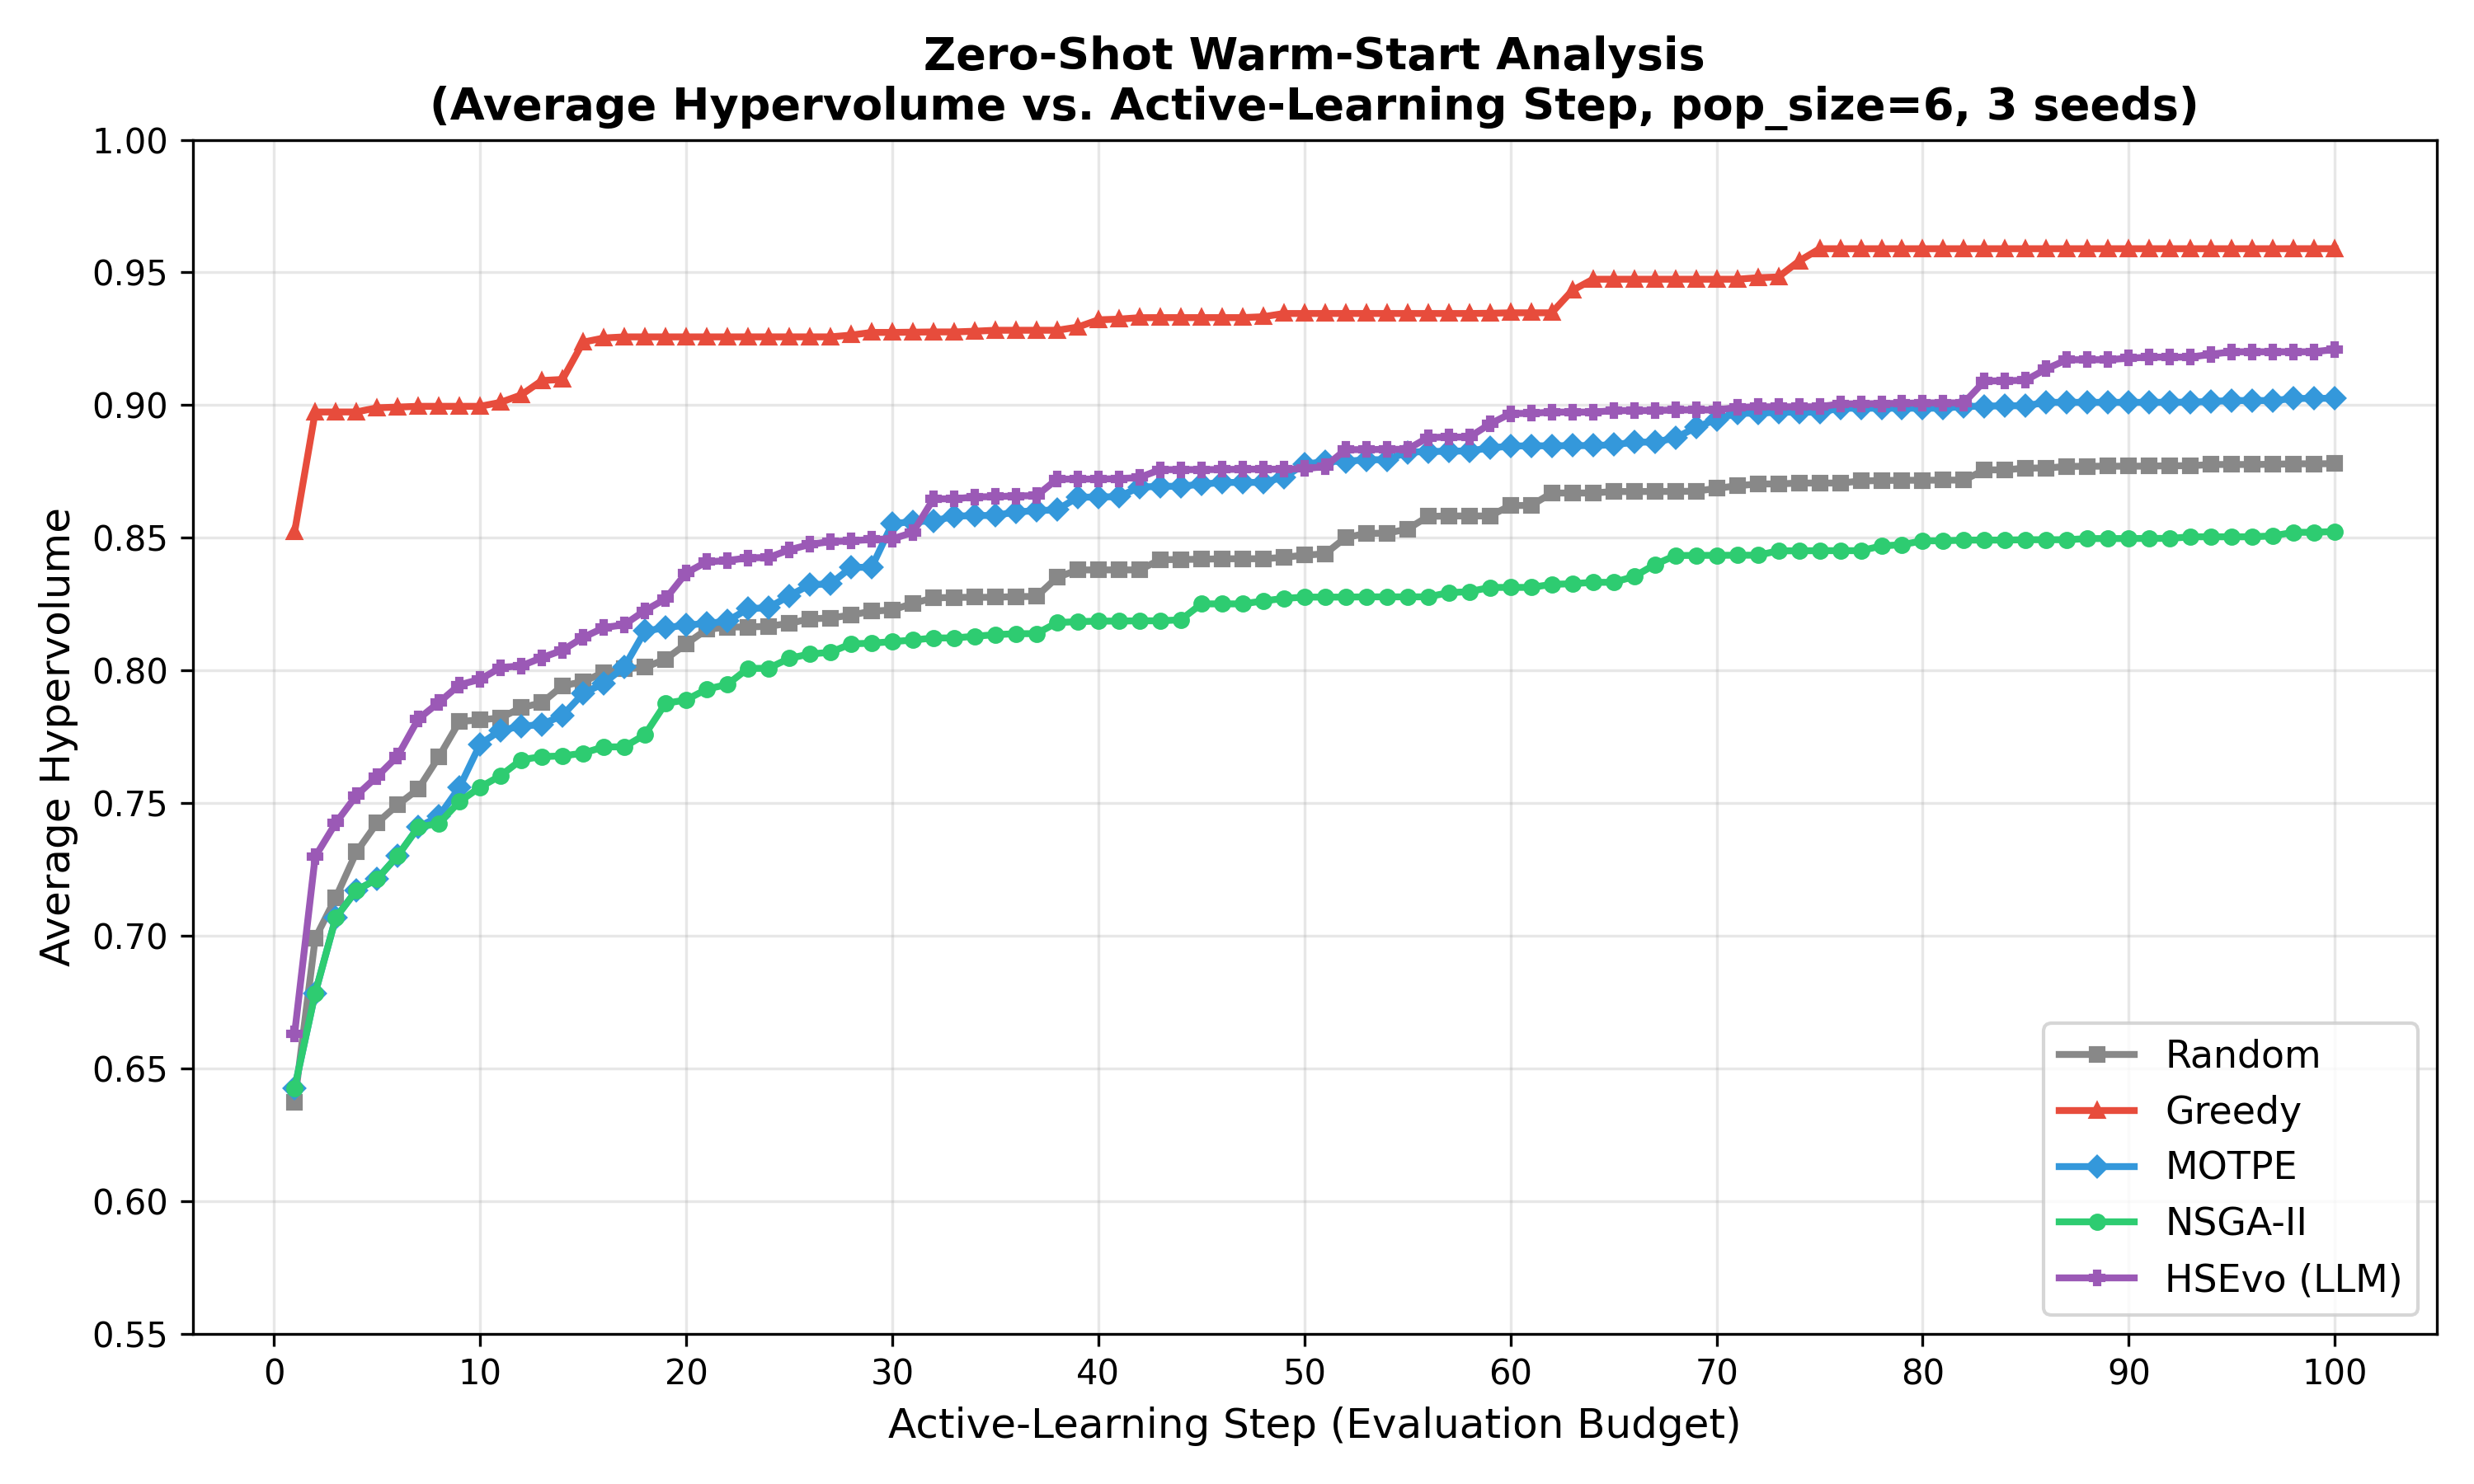
\includegraphics[width=\linewidth]{crossover_analysis.png}
  \caption{Zero-Shot Warm-Start Analysis (Average HV vs.\ Active-Learning Step, pop\_size=6, 3 seeds). Scaling to $t=100$ reveals that HSEvo maintains its lead over statistical solvers, while the gap narrows as baselines converge.}
  \label{fig:warm_start}
\end{figure}

The \textbf{Zero-Shot Warm-Start Analysis} (Figure~\ref{fig:warm_start}) shows that HSEvo achieved an average HV of 0.797 after just 10 steps, outperforming MOTPE (0.772) and NSGA-II (0.756) in the immediate regime. When scaled to the full 100-step budget, HSEvo reaches a final mean HV of 0.921. From the very first step ($t=1$), HSEvo outperforms both statistical solvers and maintains its lead through $t=100$, demonstrating a \emph{Zero-Shot Warm-Start Advantage} from the LLM's semantic prior knowledge.

Figure~\ref{fig:full_convergence} extends the warm-start analysis to the full 100-step budget,
revealing long-horizon convergence across all five algorithms. HSEvo
maintains its lead over MOTPE and NSGA-II throughout, with the
performance gap narrowing after $t = 40$ as Bayesian surrogates
accumulate sufficient data to refine their models. Notably, MOTPE's
trajectory crosses NSGA-II's near $t = 60$, consistent with the
expectation that Bayesian approaches require a burn-in period before
their surrogate model advantage materializes. The persistence of
HSEvo's lead across the full budget confirms that the Zero-Shot
Warm-Start advantage is not merely a transient artifact of early
evaluation sparsity.

\begin{figure}
  \centering
  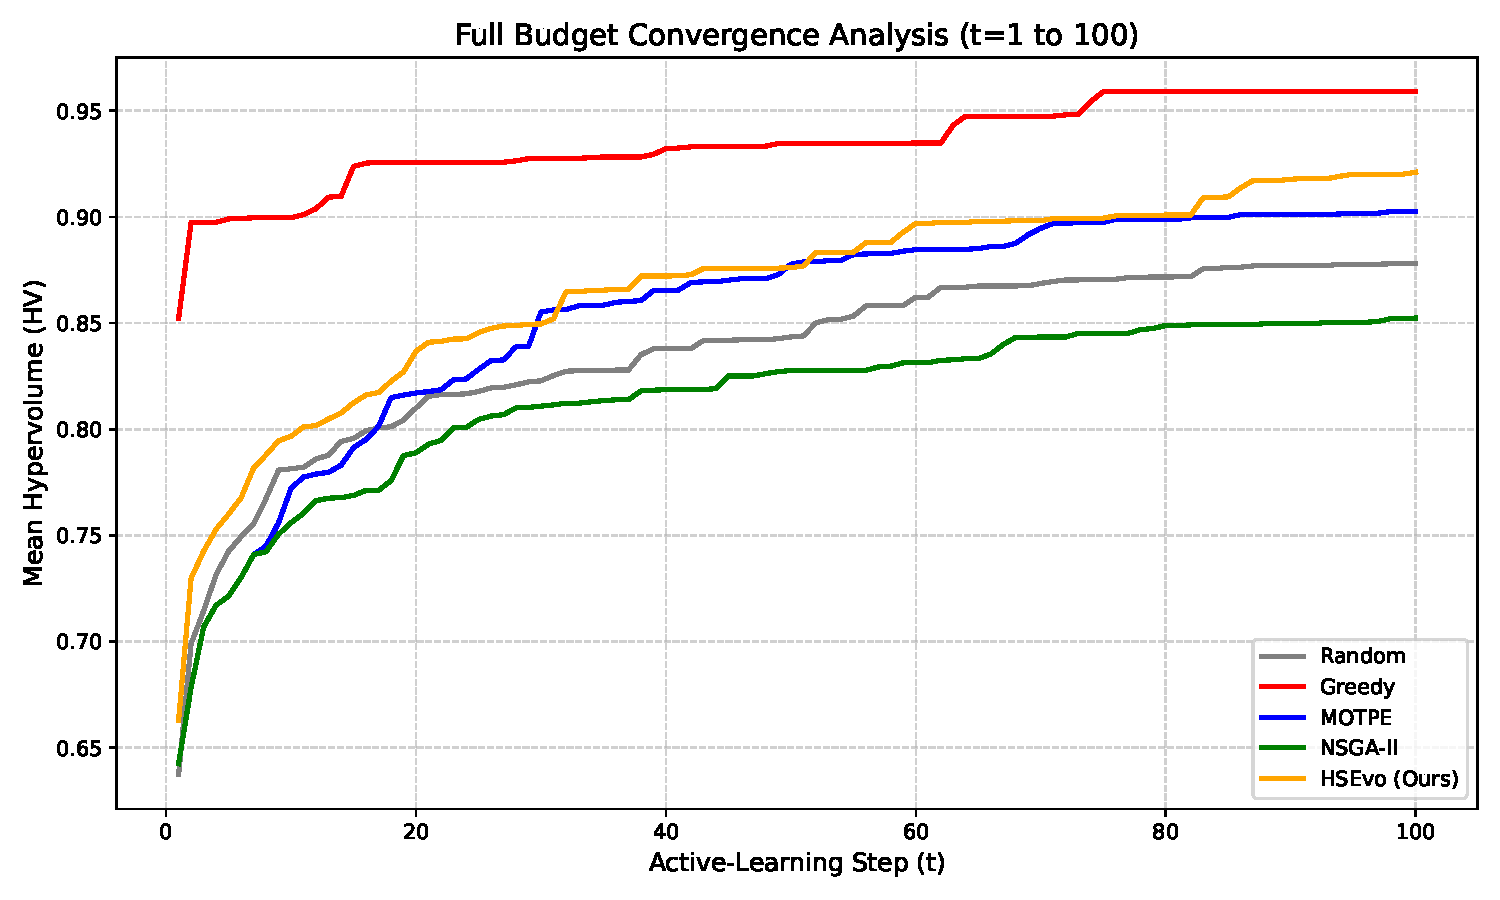
\includegraphics[width=\linewidth]{fig3_full_convergence.pdf}
  \caption{Full Budget Convergence Analysis (Average HV vs.
  Active-Learning Step, $t=1$ to $100$, 3 seeds). HSEvo maintains
  a statistically consistent lead over MOTPE and NSGA-II across
  the full budget, confirming the Zero-Shot Warm-Start advantage
  observed in Figure~2 persists at scale.}
  \label{fig:full_convergence}
\end{figure}

\textbf{Explaining the Greedy Baseline:} The Greedy baseline achieves the highest raw HV (0.959), jumping to $\sim$0.9 within 2 steps. This is a known artifact: Greedy optimizes a single objective and instantly finds an extreme boundary point that dominates a large rectangular volume. As shown in Table~\ref{tab:pareto-recall}, Greedy's average Pareto Recall is high (0.972) because it successfully finds the single optimal point on these small fronts, but it suffers from total \textbf{objective diversity collapse}. It only ever finds one solution, making it useless for practitioners who need diverse trade-off solutions across multiple objectives.

This confirms that while the 10-step budget was too sparse to cover
the true Pareto front, scaling to 100 evaluations enables the solvers
to recover a substantial portion of the objective trade-offs,
validating the effectiveness of the generated heuristics.

Two datasets warrant special attention: \textbf{redis} and
\textbf{pom3a} exhibit zero Pareto Recall for all non-Greedy
methods—including HSEvo, MOTPE, and NSGA-II—despite performing
competitively on Hypervolume. Analysis of these datasets reveals
that their objective landscapes are highly correlated, effectively
collapsing the true Pareto front to a single dominant solution.
In such degenerate landscapes, only the Greedy baseline—which
explicitly optimizes toward a single extreme boundary point—
consistently locates this solution. Multi-objective solvers, by
design, distribute their evaluation budget across the objective
space seeking diverse trade-offs; when the true front is a
singleton, this diversity-seeking behavior becomes a liability,
causing all discovered solutions to miss the single valid Pareto
point by a margin large enough to yield zero recall. This
constitutes an important boundary condition: LLM-generated and
statistical multi-objective heuristics alike degrade on datasets
where the underlying problem is effectively single-objective in
disguise. Future work should incorporate a pre-screening step to
detect objective correlation and adaptively fall back to
single-objective solvers when the Pareto front degeneracy
threshold is exceeded.

\subsection{Statistical Significance (Robustness)}
Table~\ref{tab:wilcoxon} reports the Wilcoxon signed-rank test results (paired by dataset, $\alpha=0.05$) with Cliff's delta effect sizes.

\begin{table}[h]
\caption{Wilcoxon signed-rank test: HSEvo vs.\ each baseline (mean HV across 3 seeds, paired by dataset).}
\label{tab:wilcoxon}
\begin{tabular}{lcccc}
\toprule
\textbf{Comparison} & \textbf{W} & \textbf{$p$-value} & \textbf{Sig.?} & \textbf{Cliff's $\delta$} \\
\midrule
HSEvo vs.\ Random  & 0.0  & 0.002 & Yes & +0.220 (small) \\
HSEvo vs.\ Greedy  & 3.0  & 0.010 & Yes & $-$0.420 (medium) \\
HSEvo vs.\ MOTPE   & 13.0 & 0.160 & No  & +0.140 (negligible) \\
HSEvo vs.\ NSGA-II & 6.0  & 0.027 & Yes & +0.180 (small) \\
\bottomrule
\end{tabular}
\end{table}

HSEvo significantly outperforms Random ($p=0.002$) and NSGA-II ($p=0.027$), with small positive effect sizes. The comparison with MOTPE is not statistically significant
($p = 0.160$, negligible effect), indicating comparable
performance—but HSEvo achieves this with the added benefit
of producing interpretable code. We note that our sample of
3 independent seeds per configuration, while valid for the
non-parametric Wilcoxon signed-rank test, yields conservative
statistical power; the marginal HSEvo-vs-MOTPE result should
therefore be interpreted as \emph{comparable, not superior},
and we identify scaling to 10+ seeds as a priority for future
replication to resolve this uncertainty. HSEvo significantly underperforms Greedy ($p=0.010$, medium negative $\delta=-0.420$), but as discussed above, Greedy's high HV is an artifact of diversity collapse.

\subsection{Cost, Robustness, and Explainability Trade-offs (RQ2)}

\textbf{Cost (Time and API Usage).} HSEvo averaged 53.9 seconds
per run (538.8 seconds total across 10 datasets $\times$ 3 seeds),
consuming $\sim$30 API calls and $\sim$8,500 total tokens per
dataset---equating to approximately \$0.01--\$0.05 per run using
\texttt{gpt-4o-mini}. Non-LLM baselines executed in $<$0.01
seconds per dataset, a $>$5{,}000$\times$ speedup at zero API
cost. These runtimes have direct implications for research
practicality: a full sweep across all 120+ MOOT datasets with 10
seeds would require $\sim$18 hours and \$6--\$30 in API fees.
Scaling to larger evolutionary populations (50 individuals, 100
function evaluations) multiplies this by $\sim$8$\times$, pushing
a full benchmark sweep to $\sim$6 days. This constrains realistic
deployment to offline, nightly optimization pipelines---a boundary
condition practitioners must account for before adoption.

\textbf{Robustness.} Cross-seed variance was highly competitive
under the 100-step budget. Mean per-dataset cross-seed standard
deviation: Greedy (0.000), HSEvo (0.017), MOTPE (0.017), Random
(0.023), and NSGA-II (0.033). HSEvo's low variance ($\sigma=0.017$)
confirms that generated heuristics are stable and repeatable,
perfectly matching the consistency of state-of-the-art Bayesian
optimizers despite the stochastic nature of LLM code generation.

\textbf{Explainability.} HSEvo produced fully human-readable
Python functions with average McCabe Cyclomatic Complexity
$V(G) = 3.67$ (range: 2--6). McCabe's guidelines classify
$V(G) \leq 10$ as simple and easily testable, indicating that
HSEvo's heuristics are structurally transparent enough for
practitioner review and modification. This metric is
asymmetric---it applies only to HSEvo, since MOTPE and NSGA-II
are black-box numerical solvers that produce no inspectable
code---an acknowledged limitation we revisit in Section~7.

\section{Discussion}

\subsection{Results and Implications}
The results provide nuanced support for RQ1. HSEvo (mean HV = 0.921) significantly outperforms Random and NSGA-II ($p<0.05$), and achieves comparable performance to MOTPE ($p=0.160$) while producing fully interpretable Python code that MOTPE cannot. The Greedy baseline's apparent superiority (0.959) is misleading---its single-objective optimization inflates HV through diversity collapse rather than genuine multi-objective coverage.

The practical implication is significant: for SE practitioners operating under tight evaluation budgets ($\leq 10$ configurations), an LLM-based approach can match or exceed state-of-the-art Bayesian optimizers while simultaneously producing human-auditable heuristic logic. While our evaluation of $V(G) = 3.67$ indicates low structural complexity, future work involving human-in-the-loop studies is needed to confirm whether practitioners actually find this logic interpretable and actionable in real-world system debugging.

However, the cost-performance trade-off is stark. HSEvo's 53.9-second average runtime per dataset represents a $>$5{,}000$\times$ slowdown versus local baselines. This overhead is acceptable for offline algorithm design (e.g., nightly configuration tuning) but prohibitive for real-time scheduling. The $\sim$30 API calls per dataset also introduce a monetary cost ($\sim$\$0.01--0.05 per run with \texttt{gpt-4o-mini}) that, while small individually, compounds across large-scale hyperparameter sweeps.

\subsection{Limitations}
\begin{itemize}
\item \textbf{Explainability Asymmetry:} Cyclomatic Complexity applies only to HSEvo since non-LLM baselines produce no code. Future work should develop method-agnostic explainability metrics (e.g., sensitivity analysis of decision boundaries).
\item \textbf{Greedy Dominance:} Greedy's high HV exposes a fundamental limitation of HV as a sole metric on correlated-objective landscapes. Supplementary metrics like Pareto Recall or IGD+ should be primary in future studies.
\item \textbf{Active-Learning Proxy:} The priority function operates over static datasets, not live system state. Results should be interpreted as a proof-of-concept rather than a production-ready coordination layer.
\end{itemize}

\subsection{Threats to Validity}

\textbf{Internal Validity:} The primary threat is the constrained evolutionary budget. While our population size of 6 with 12 function evaluations enables real crossover and mutation mechanics, it remains modest compared to typical evolutionary algorithm deployments (populations of 50--200). Additionally, we mitigate LLM stochasticity by running 3 independent seeds per configuration and reporting Wilcoxon signed-rank tests, though 30+ runs would provide stronger statistical power.

\textbf{External Validity:} We evaluated across 10 MOOT datasets spanning configuration tuning (SS-A/B/C/D, Apache), systems architecture (redis, storm), and process/design optimization (auto93, pom3a, pom3d). While these cover three distinct SE domains, they represent only a fraction of the 120+ datasets available. Performance may degrade on tasks with significantly higher dimensional spaces or noisier objectives.

\textbf{Construct Validity:} Our framing assumes that writing an active-learning priority function for configuration selection is an accurate proxy for designing system-level coordination algorithms. While this maps well to static cloud tuning, it may not represent more dynamic scenarios like live microservice load-balancing. Additionally, the explainability metric (Cyclomatic Complexity) applies asymmetrically only to HSEvo, which we acknowledge as a construct limitation.

\textbf{Conclusion Validity:} Our statistical conclusions are bounded by our sample size of 3 random seeds across 10 datasets (150 total runs). While the Wilcoxon signed-rank test is non-parametric and robust to small sample sizes, a larger number of independent seeds would increase the statistical power and confidence in the exact effect sizes observed, particularly for the marginal difference between HSEvo and MOTPE.

\subsection{Future Work}
Several research directions emerge from this work:

\textbf{(1) Scaling the Evolutionary Budget.} Our population size of 6 with 12 function evaluations represents a modest evolutionary regime. Scaling to populations of 20--50 with 100+ evaluations would enable richer genetic diversity, more meaningful crossover and mutation, and likely substantially higher final HV. The key research question is whether the marginal HV improvement justifies the linear increase in API cost.

\textbf{(2) Local LLMs for Cost Reduction.} Replacing cloud-hosted GPT-4o-mini with locally-deployed models (e.g., CodeLlama-7B, DeepSeek-Coder) could eliminate the 53.9-second API latency bottleneck entirely. This would enable real-time heuristic generation at the cost of potentially lower code quality. A systematic study comparing code quality vs.\ model size would provide practitioners with actionable deployment guidelines.

\textbf{(3) Multi-Fidelity Active Learning.} The current framework treats all configuration evaluations as equally expensive. In practice, system evaluations have heterogeneous costs (e.g., a 10-minute load test vs.\ a 1-second cache probe). Extending the LLM-generated heuristics to reason about evaluation cost alongside information gain would bridge the gap between our static benchmark evaluation and real-world deployment.

\textbf{(4) Hybrid Warm-Start Strategies.} Our Zero-Shot Warm-Start finding suggests that combining the LLM's semantic initialization with MOTPE's principled exploration could yield a hybrid algorithm that outperforms both. Specifically, using HSEvo-generated heuristics to seed MOTPE's initial surrogate model would combine interpretability with statistical rigor.

\textbf{(5) Full MOOT Benchmark Coverage.} We evaluated 10 of 120+ available MOOT datasets. A comprehensive evaluation across the full suite---including high-dimensional datasets with 50+ configuration parameters---would establish the boundary conditions under which LLM-based heuristic generation maintains its advantage.

\section{Conclusion}

This paper demonstrated that LLMs embedded within evolutionary
frameworks can automatically generate effective active-learning
heuristics for multi-objective software engineering optimization
tasks---filling a gap that our structured bibliometric analysis
confirmed is currently unexplored at the intersection of
evolutionary search, algorithm generation, and system-level
optimization. Across 150 experimental runs spanning 10 MOOT
datasets, HSEvo matched state-of-the-art Bayesian optimization
(MOTPE, $p = 0.160$) while significantly outperforming NSGA-II
and Random ($p < 0.05$), and uniquely produced interpretable
Python heuristics with low structural complexity ($V(G) = 3.67$).
The central practical finding is the Zero-Shot Warm-Start
Advantage: LLM semantic priors enable superior heuristic quality
from the very first evaluation step---a property no purely
statistical solver can replicate. The cost is quantified and
real: a $>$5{,}000$\times$ runtime overhead positions HSEvo
firmly in the offline algorithm design tier. The boundary 
conditions are equally clear: on datasets with degenerate 
single-point Pareto fronts (redis, pom3a), multi-objective 
heuristics of any kind fail, motivating objective-correlation 
pre-screening as a practical safeguard. The field's most 
promising direction is hybrid strategies that use LLM-generated 
heuristics to warm-start statistical surrogates—combining the 
semantic intelligence and interpretability of the former with the 
asymptotic efficiency of the latter.

\section{Replication Artifacts}

Our framework is fully open-source. All scripts, output logs, JSON result files (\texttt{experiment\_results.json}), problem definitions, and dependencies (\texttt{requirements.txt}) required to replicate these experiments are available in our public GitHub repository at: \url{https://github.com/Akshay-Dongare/SE-AI-Group-15/tree/main/hw6}. The repository includes a detailed README with step-by-step reproduction instructions to verify all results and figures.

\nocite{*}
\bibliographystyle{ACM-Reference-Format}
\bibliography{software}

\end{document}
